\documentclass[portrait,b1paper,fontscale=0.400]{baposter}

\usepackage[brazil]{babel}
\usepackage[utf8]{inputenc}
\usepackage[vlined]{algorithm2e}
\usepackage{times}
\usepackage{calc}
\usepackage{url}
\usepackage{graphicx}
\usepackage{amsmath}
\usepackage{amssymb}
\usepackage{relsize}
\usepackage{multirow}
\usepackage{booktabs}
\usepackage{graphicx}
\usepackage{multicol}
\usepackage[T1]{fontenc}
\usepackage{ae}

\graphicspath{{fig/}}

% Multicol Settings
\setlength{\columnsep}{0.7em}
\setlength{\columnseprule}{0mm}

% Formating
\newcommand*{\norm}[1]{\mathopen\| #1 \mathclose\|}
\newcommand*{\abs}[1]{\mathopen| #1 \mathclose|}
\newcommand*{\dd}{\partial}
\newcommand*{\VEC}[1]  {\ensuremath{\boldsymbol{#1}}}
\newcommand*{\CONST}[1]{\ensuremath{\mathit{#1}}}
\renewcommand*{\d}{\mathrm{d}}
\DeclareMathOperator*{\argmax}{arg\,max}

% Estilo dos parágrafos
% \sloppy                              % Mais flexível
% \setlength{\jot}{08pt}               % Distância entre linhas do eqnarray
% \setlength{\parskip}{1ex}            % Distância entre parágrafos
% \renewcommand{\baselinestretch}{1.0} % Distância entre linhas

% Comandos customizados
\newcommand{\vet}{\mathbf}                                   % vetor
\newcommand{\ie}{\emph{i.e.}}                                % isto é
\newcommand{\prodint}[2]{\left\langle #1 , #2 \right\rangle} % produto interno
\newcommand{\Fullbox}{{\rule{2.0mm}{2.0mm}}}                 % caixa cheia
\newcommand{\EOS}{\hfill\Box\vspace{-0.2cm}}                 % fim de enunciado
\newcommand{\EOP}{\hfill\Fullbox\vspace{0.2cm}}              % fim de prova
\newcommand{\eps}{\varepsilon}                               % epsilon
\newcommand{\defi}{\: := \: }                                % definição
\newcommand{\del}{\partial}                                  % derivada parcial
\newcommand{\hsp}{\hspace{0.5cm}}                            % espaco horizontal para fórmulas
\newcommand{\vsp}{\vspace{0.1cm}}                            % espaco vertical para fórmulas
\newcommand{\ev}{\, ,}                                       % espaco e virgula
\newcommand{\ep}{\, .}                                       % espaco e ponto
\newcommand{\eg}{\emph{e.g.}}                                % por exemplo

\begin{document}
\begin{poster}{
columns=3,
% Show grid to help with alignment
grid=false,
% Column spacing
colspacing=0.7em,
% Color style
headerColorOne=cyan!20!white!90!black,
borderColor=cyan!30!white!90!black,
% Format of textbox
textborder=rounded,
boxshade=none,
% Format of text header
headerborder=open,
headershape=roundedright,
headershade=plain,
background=none,
bgColorOne=cyan!10!white,
headerheight=0.12\textheight}
% Eye Catcher
{
 
\includegraphics[height=0.060\textheight]{gol}
}
% Title
{
\sc\Huge Otimização de Viagens em Companhias \\ Aéreas Brasileiras
}
% Authors
{
Daniel Augusto Cortez, Lucas Rodrigues Colucci e Renato Lerac Corrêa de Sá\\[1em]
{\texttt{dacortez79@gmail.com, lucasrcolucci@gmail.com, renatolerac@gmail.com}}
}
% University logo
{
 
\includegraphics[height=0.095\textheight]{logo}
}


%%%%%%%%%%%%%%%%%%%%%%%%%%%%%%%%%%%%%%%%%%%%%%%%%%%%%%%%%%%%%%%%%%%%%%%%%%%%%%
\headerbox{Introdução}{name=introducao,column=0,row=0}{
%%%%%%%%%%%%%%%%%%%%%%%%%%%%%%%%%%%%%%%%%%%%%%%%%%%%%%%%%%%%%%%%%%%%%%%%%%%%%%
As tripulações de uma companhia aérea representam o segundo maior custo operacional, perdendo apenas 
para o combustível. Um processo otimizado de escalonamento pode resultar em ganhos econômicos da 
ordem de milhões de dólares.

O problema é resolvida em duas etapas. Na primeira delas, determina-se uma partição dos voos da 
empresa em um conjunto de viagens legais de custo mínimo (PDV). Na segunda, as viagens obtidas devem 
ser atribuídas aos tripulantes de forma a minimizar os custos (PDE).

Estudamos aqui o PDV. Uma viagem é definida como uma sequencia de voos encadeados no espaço e no 
tempo, obedecendo uma série de restrições legais impostas pela legislação do aeronauta 
{\bf brasileira}, originando e terminando na base residencial do tripulante.
%
\begin{center}
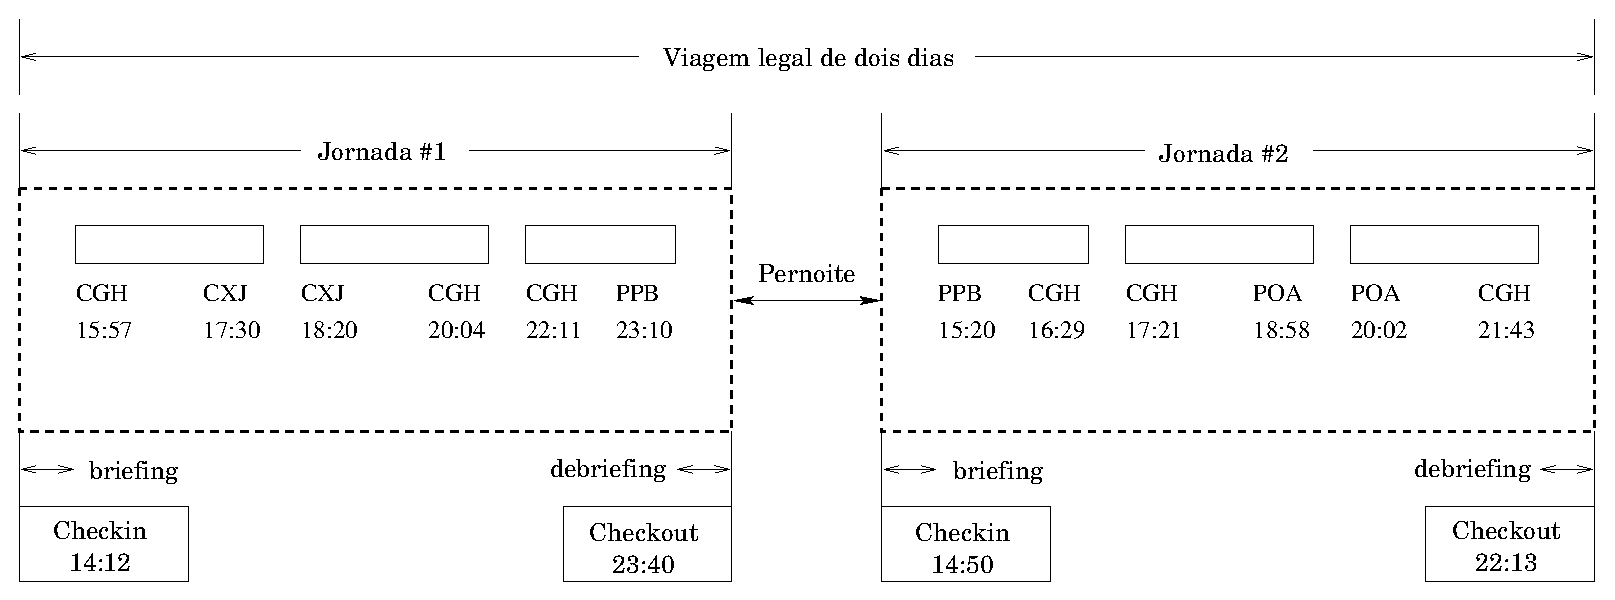
\includegraphics[width=0.99\linewidth]{pairing}
\end{center}
%
Implementamos e comparamos três métodos de solução do PDV: um algoritmo baseado em uma busca 
local, um algoritmo genético híbrido e um procedimento de geração de colunas.
}

%%%%%%%%%%%%%%%%%%%%%%%%%%%%%%%%%%%%%%%%%%%%%%%%%%%%%%%%%%%%%%%%%%%%%%%%%%%%%%
\headerbox{Formulação}{name=formulacao,column=0,below=introducao}{
%%%%%%%%%%%%%%%%%%%%%%%%%%%%%%%%%%%%%%%%%%%%%%%%%%%%%%%%%%%%%%%%%%%%%%%%%%%%%%
O PDV pode ser formulado como um problema de programação linear inteiro conhecido por 
{\bf Set Cover}: Seja $x_j = 1$ se a viagem $j$ for escolhida, com custo $c_j$. Seja $y_i \geq 0$ o 
número de vezes que o voo $i$ é coberto e $d_i$ o custo associado. Então, queremos resolver:
%
\begin{eqnarray*}
	\text{minimizar} && \displaystyle \sum_{j=1}^n c_j x_j + \sum_{i=1}^m d_i y_i \\
	\text{sujeito à} && \displaystyle \sum_{j=1}^n a_{ij} x_j - y_i = 1 \ev \;\; i = 1, \ldots, m \\
	                 && x_j \in \{0, 1\} \ev \;\; j = 1, \ldots, n \\
	                 && y_i \geq 0 \ev \;\; i = 1, \ldots, m \ep
\end{eqnarray*}
%
Dado que o problema é NP-difícil e que existe um número enorme de variáveis (viagens possíveis), 
métodos heurísticos devem ser aplicados.
}


%%%%%%%%%%%%%%%%%%%%%%%%%%%%%%%%%%%%%%%%%%%%%%%%%%%%%%%%%%%%%%%%%%%%%%%%%%%%%%
\headerbox{Geração de Viagens}{name=geracao,column=0,below=formulacao,above=bottom}{
%%%%%%%%%%%%%%%%%%%%%%%%%%%%%%%%%%%%%%%%%%%%%%%%%%%%%%%%%%%%%%%%%%%%%%%%%%%%%%
As viagens para otimização são geradas a partir de uma {\bf busca em profundidade} na rede de voos 
do problema. Cada nó representa um voo e arcos são adicionados toda vez que for possível estabelecer 
uma conexão legal entre os voos. Uma fonte $s$ e um sorvedouro $t$ são adicionados e os voos que se 
iniciam na base da tripulação são ligados à $s$. Os voos que chegam na base são ligados à $t$. Toda 
viagem viável representa um caminho $s-t$ no grafo.
%
\begin{center}
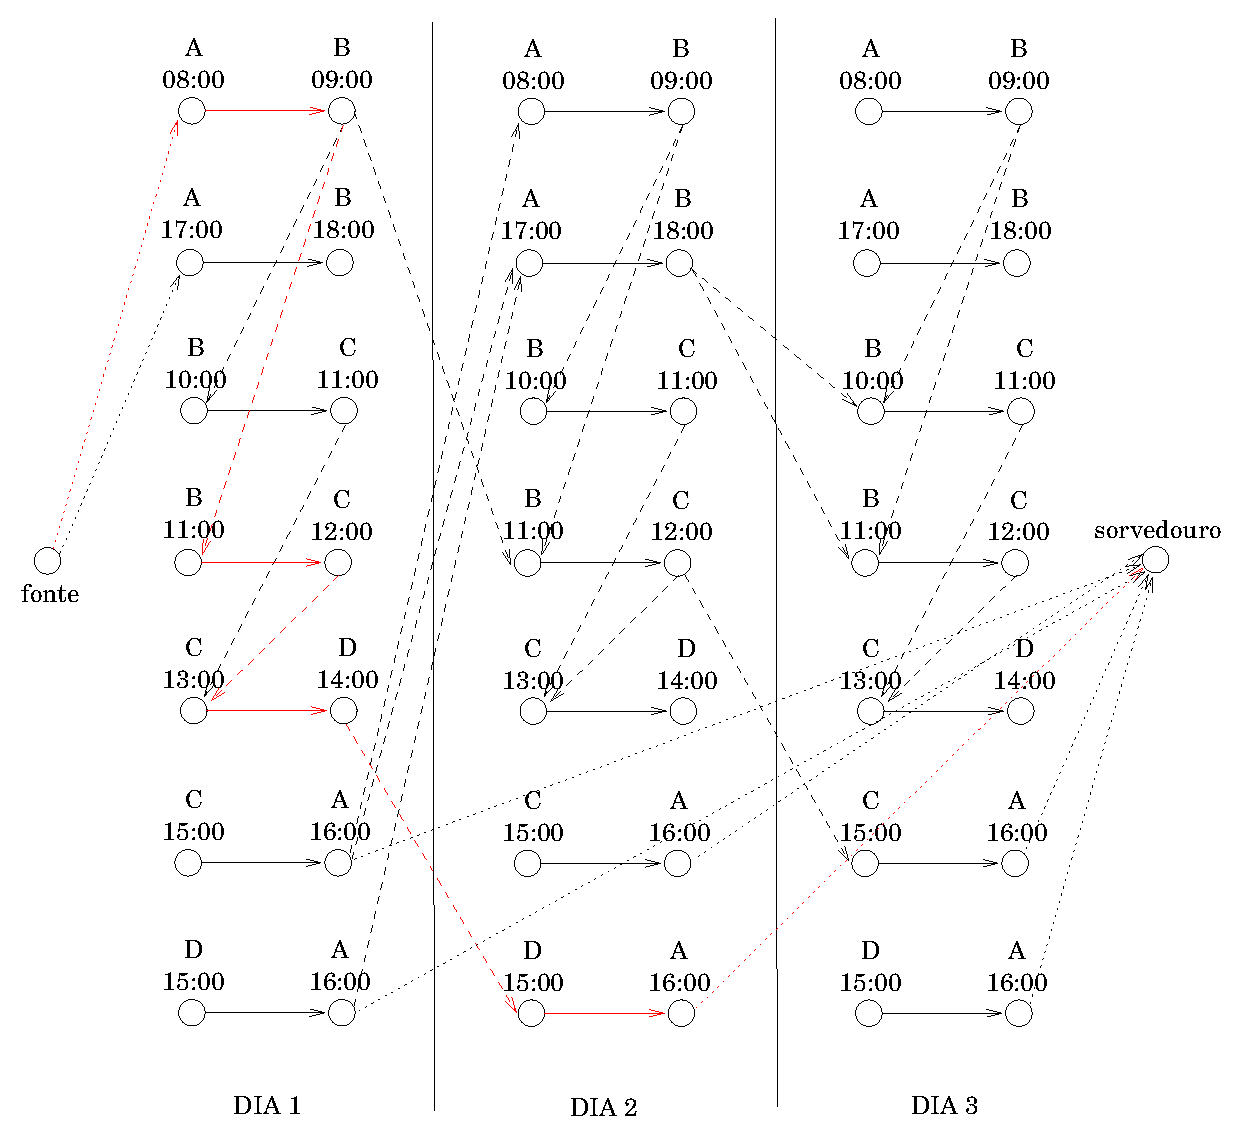
\includegraphics[width=0.98\linewidth]{network}
\end{center}
}


% %%%%%%%%%%%%%%%%%%%%%%%%%%%%%%%%%%%%%%%%%%%%%%%%%%%%%%%%%%%%%%%%%%%%%%%%%%%%%%
% \headerbox{Referencias}{name=referencias,column=0,below=geracao,above=bottom}{
% %%%%%%%%%%%%%%%%%%%%%%%%%%%%%%%%%%%%%%%%%%%%%%%%%%%%%%%%%%%%%%%%%%%%%%%%%%%%%%
% \smaller   
% \bibliographystyle{ieee}
% \renewcommand{\section}[2]{\vskip 0.05em}
% \begin{thebibliography}{1}\itemsep=-0.01em
%  \setlength{\baselineskip}{0.4em}
%  \bibitem{crew_pairings} 
% \end{thebibliography}
% }


%%%%%%%%%%%%%%%%%%%%%%%%%%%%%%%%%%%%%%%%%%%%%%%%%%%%%%%%%%%%%%%%%%%%%%%%%%%%%%
\headerbox{Análise Preliminar}{name=preliminar,column=1,row=0}{
%%%%%%%%%%%%%%%%%%%%%%%%%%%%%%%%%%%%%%%%%%%%%%%%%%%%%%%%%%%%%%%%%%%%%%%%%%%%%%
Resolvemos exatamente o PLI para um conjunto de voos utilizando os otimizadores GLPK e CPLEX. 
Dado o número enorme de variáveis geradas, os problemas não puderam ser resolvidos em tempo hábil 
mesmo para um número pequeno de pernas (voos).
\begin{center}
\includegraphics[width=0.92\linewidth]{preliminary}
\end{center}
}


%%%%%%%%%%%%%%%%%%%%%%%%%%%%%%%%%%%%%%%%%%%%%%%%%%%%%%%%%%%%%%%%%%%%%%%%%%%%%%%
\headerbox{Busca Local}{name=local,column=2,row=0}{
%%%%%%%%%%%%%%%%%%%%%%%%%%%%%%%%%%%%%%%%%%%%%%%%%%%%%%%%%%%%%%%%%%%%%%%%%%%%%%%
\begin{center}
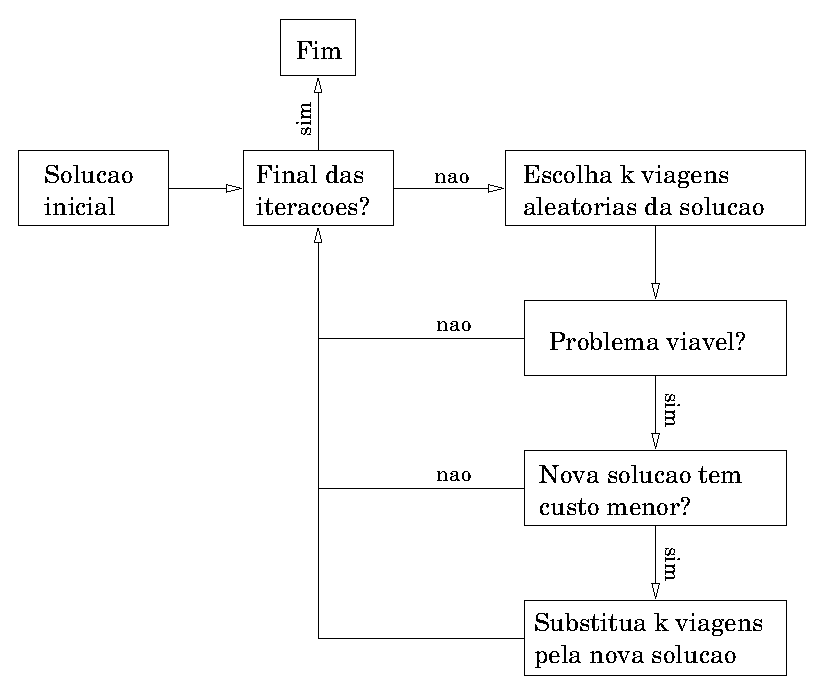
\includegraphics[width=0.90\linewidth]{local}
\end{center}
}


%%%%%%%%%%%%%%%%%%%%%%%%%%%%%%%%%%%%%%%%%%%%%%%%%%%%%%%%%%%%%%%%%%%%%%%%%%%%%%
\headerbox{Algoritmo Genético}{name=genetico,column=1,below=preliminar}{
%%%%%%%%%%%%%%%%%%%%%%%%%%%%%%%%%%%%%%%%%%%%%%%%%%%%%%%%%%%%%%%%%%%%%%%%%%%%%%
\begin{algorithm}[H]
 \dontprintsemicolon
 %\linesnumbered
 \For{Blur and regularisation values}{
  Initialize $q, q_{\text{best}}$ and $\kappa$\;
 \Repeat{converged}{
  Calculate $\Delta{p}{\tilde{F}(q, 0)}$, $F(q)$\;
  \eIf{$F(q) < F(q_{\text{best}})$}{
    %\nl Calculate distance between best warp estimate and current warp estimate to test for convergence\;
    $q_{\text{best}} \gets q$\;
    %\If{More than three successiv updates}{ (Too much detail)
    Increase $\kappa$\;
    %}
 }{
   \If{$\kappa$ smaller than threshold}{
     return\;
    }%{
       decrease $\kappa$\;
    %}
  }
  Calculate $p$ from $\Delta{p}{\tilde{F}(q_{best},p)}$ and $\kappa$\;
  $q \gets C{\circ}{q, p}$
 }
}
\end{algorithm}
}


%%%%%%%%%%%%%%%%%%%%%%%%%%%%%%%%%%%%%%%%%%%%%%%%%%%%%%%%%%%%%%%%%%%%%%%%%%%%%%
\headerbox{Geração de Colunas}{name=cg,column=2,below=local}{
%%%%%%%%%%%%%%%%%%%%%%%%%%%%%%%%%%%%%%%%%%%%%%%%%%%%%%%%%%%%%%%%%%%%%%%%%%%%%%
\begin{algorithm}[H]
\dontprintsemicolon
$\VEC{x} \gets$ solução viável\;
	$\VEC{\pi} \gets $ duais da relaxação com \VEC{x}  
\Repeat{$w^\star$ > 0}{

}
\For{Blur and regularisation values}{
  Initialize $q, q_{\text{best}}$ and $\kappa$\;
 \Repeat{converged}{
  Calculate $\Delta{p}{\tilde{F}(q, 0)}$, $F(q)$\;
  \eIf{$F(q) < F(q_{\text{best}})$}{
    %\nl Calculate distance between best warp estimate and current warp estimate to test for convergence\;
    $q_{\text{best}} \gets q$\;
    %\If{More than three successiv updates}{ (Too much detail)
    Increase $\kappa$\;
    %}
 }{
   \If{$\kappa$ smaller than threshold}{
     return\;
    }%{
       decrease $\kappa$\;
    %}
  }
  Calculate $p$ from $\Delta{p}{\tilde{F}(q_{best},p)}$ and $\kappa$\;
  $q \gets C{\circ}{q, p}$
 }
}
\end{algorithm}
}


%%%%%%%%%%%%%%%%%%%%%%%%%%%%%%%%%%%%%%%%%%%%%%%%%%%%%%%%%%%%%%%%%%%%%%%%%%%%%%
\headerbox{Conclusões}{name=conclusoes,column=1,span=2,above=bottom}{
%%%%%%%%%%%%%%%%%%%%%%%%%%%%%%%%%%%%%%%%%%%%%%%%%%%%%%%%%%%%%%%%%%%%%%%%%%%%%%

}

%%%%%%%%%%%%%%%%%%%%%%%%%%%%%%%%%%%%%%%%%%%%%%%%%%%%%%%%%%%%%%%%%%%%%%%%%%%%%%
\headerbox{Resultados}{name=resultados,column=1,span=2,below=genetico,above=conclusoes}{
%%%%%%%%%%%%%%%%%%%%%%%%%%%%%%%%%%%%%%%%%%%%%%%%%%%%%%%%%%%%%%%%%%%%%%%%%%%%%%
\centering
\includegraphics[width=0.98\linewidth]{results}

\begin{center}
\vspace{0.2cm}
\scalebox{0.98}{
\begin{tabular}{cc|c|c|c|c|c|c|c|c|c|c|}
	\cline{3-12}
	& &
	\multicolumn{2}{|c|}{73H\_26} & 
	\multicolumn{2}{|c|}{738\_48} & 
	\multicolumn{2}{|c|}{733\_92} & 
	\multicolumn{2}{|c|}{73G\_340} & 
	\multicolumn{2}{|c|}{cgh\_sdu\_62} \\
	\cline{3-12}
	& & Obj & CPU & Obj & CPU & Obj & CPU & Obj & CPU & Obj & CPU \\

	\hline
	\multicolumn{2}{|c|}{CG} & 
	5,696  & 0,26  & 
	6,230  & 0,54  & 
	10,973 & 1,36  & 
	42,744 & 54,02 & 
	10,103 & 1,13 \\

	\hline
	\multicolumn{1}{|c|}{\multirow{3}{*}{LS}} 
	& $k = 2$ & 
	0\%    & 1,10   & 
	>100\% & 1,22   & 
  >100\% & 3,16   & 
	>100\% & 208,44 & 
	>100\% & 0,79 \\
	\multicolumn{1}{|c|}{} 
	& $k = 3$ & 
	0\%    & 1,48    & 
	14,1\% & 7,91    & 
	8,1\%  & 18,68   & 
	32,5\% & 1303,53 & 
	87,9\% & 1,31 \\
	\multicolumn{1}{|c|}{} 
	& $k = 4$ & 
	0\%    & 1,81 & 
	0\%    & 11,46 & 
	8,0\%  & 99,09 & 
	25,7\% & 2182,31 & 
	0\%    & 17,83 \\

	\hline
	\multicolumn{1}{|c|}{\multirow{3}{*}{AG}} 
	& $f = 1$ & 
	0\%    & 1,39 & 
	78,1\% & 4,35 & 
	>100\% & 8,30 & 
	>100\% & 1074,97 & 
	56,2\% & 4,31 \\
	\multicolumn{1}{|c|}{} 
	& $f = 5$ & 
	0\%    & 4,17 & 
	13,8\% & 13,19 & 
	46,4\% & 10,79 & 
	>100\% & 763,19 & 
	36,2\% & 13,99 \\
	\multicolumn{1}{|c|}{} 
	& $f = 10$ & 
	0\% & 11,01 & 
	0\% & 33,99 & 
	72,2\% & 17,85 & 
	>100\% & 482,10 & 
	30,5\% & 27,50 \\
	\hline
\end{tabular}
}
\end{center}
}

\end{poster}
\end{document}
